\chapquote{"Video killed the radio star."}{The Buggles}{1979}

\section{Introduction}

\section{The Far-Infrared/Radio Correlation}

For samples of star forming galaxies in the local and high redshift universe there is a well observed correlation between the far-infrared and radio emission (e.g. \citealt{Dickey_1984}; \citealt{deJong_1985}; \citealt{Helou_1985}; \citealt{Condon_1992}; \citealt{Barger_2000}; \citealt{Yun_2001}; \citealt{Garrett_2002}; \citealt{Appleton_2004}; \citealt{Ibar_2008}; \citealt{Seymour_2009}; \citealt{Sargent_2010}), that remains nearly linear over multiple orders of magnitude in far-infrared luminosity ($10^{9} \lesssim L_{\textrm{FIR}} [L_{\odot}] \lesssim 10^{12.5}$). The small scatter in this relation is often attributed to the "calorimeter model" (\citealt{Voelk_1989}; \citealt{Lisenfeld_1996}; \citealt{Lacki_2010}), which ascribes the far-infrared and radio emission to common stellar sources. In this model, galaxies are assumed to be opaque to UV light from massive OB stars which gets absorbed by the dust in the ISM and reradiated in the far-infrared. Observations in the far-infrared and sub-mm are thus sensitive to the cold dust that reradiates the energy from young stars. These stars quickly come to the end of their lives, exploding as Type II supernovae producing cosmic ray electrons and positrons. Most of their energy gets radiated in the radio as synchrotron radiation when interacting with the magnetic fields of the supernova remnant. The radio continuum is therefore a tracer of recent, obscured star formation.

Despite a higher scatter for high redshift SMGs than with local samples, the far-infrared/radio correlation (FIRC) still holds at increasing redshift (\citealt{Ivison_2010a}; \citealt{Ivison_2010b}). {\color{red}Small description on evolution of FIRC with redshift.}

The appearance of a correlation at all redshifts and luminosities has facilitated studies that use the radio emission as an unbiased tracer of obscured star formation in dusty galaxies (\citealt{Kennicutt_2012}). By making use of the tight correlation (as well as the benefits we outline in the following section), we can identify counterparts to single dish sub-mm observations with large beams with greater confidence than we would expect from the optical or near-infrared. This allows for better characterization of the properties of SMGs and allows us to study the cosmic star formation history to higher redshifts (\citealt{Madau_2014}; \citealt{Delhaize_2017}; \citealt{Novak_2017}).

\section{Identifying Multiwavelength Counterparts to SMGs via Radio IDs}

As illustrated in Chapter \ref{chapter:Data_Release_3}, SMGs that are detected with single dish sub-mm telescopes with low angular resolution will likely include multiple galaxies in the optical or near-infrared within the beam width. This is a particular problem for \textit{Herschel} where even the smallest beam size at 250\,\micron\ has a FWHM of $\sim$ 18 arcsec. The possibility of tightly clustered SMGs (\citealt{Blain_2004}) and with a higher surface density of optical counterparts, deciding unambiguously on the source of the sub-mm emission is difficult. This is further compounded by their intrinsic faintness due to the dust obscuration. The optimal way to overcome the problem of poor resolution is to follow up with millimetric or longer wavelength interferometric observations. In the following sections we detail a method for identifying radio counterparts to \textit{Herschel} sources in order to secure unambiguous multiwavelength counterparts to our sub-mm galaxies. The following is a list of benefits of using the radio emission to select counterparts throughout the electromagnetic spectrum.

\begin{enumerate}
    \item Star forming galaxies produce a lot of synchrotron emission. This allows us to take advantage of the FIRC to locate the galaxy emitting radiation in the far-IR. Compared to searches in other wavelengths, such as using the Likelihood Ratio to identify optical counterparts, the search for identifications is not solely motivated by their position and brightness, but also by the physical link between the two objects due to their common source.
    \item Even when considering the deepest radio maps, the low surface density of radio sources means that the probability of chance positoinal coincidences with a sub-mm source is relatively unlikely. As a result, we can have a reasonable confidence in some association between objects when we do observe radio sources in close proximity to the sub-mm position (\citealt{Ivison_2002}; \citealt{Borys_2004}). In most cases (as we shall validate in this study), radio sources are sufficiently rare that finding an object within the positional uncertainty of the sub-mm beam almost always results in a robust identification.
    \item When a secure radio counterpart is identified, the positional accuracy ($\sim$ 1 arcsec for the Karl G. Jansky Very Large Array (VLA) at 1.4\,GHz and $\sim$ 0.75 arcsec at 3\,GHz) allows for a unambiguous identification with an optical or infrared galaxy counterpart. By locating these galaxies via the radio identification, we predict a low false identification rate of the SMG with the optical counterpart, allowing us to determine their morphologies, colours, magnitudes, stellar masses and more with greater confidence.
\end{enumerate}

While the radio emission from star-forming galaxies allows for secure identification of counterparts across the spectrum, it also has several drawbacks. The following is a list of disadvantages to using radio emission.

\begin{enumerate}
    \item Our understanding of the radio-selected SMG population is likely to be skewed by selection effects. The negative k-correction in the far-infrared arises due to the steep Rayleigh-Jeans part of the SED and allows for nearly equal detection of dusty galaxies at $z \sim 0.5$ as $z \sim 8$ for longer wavelengths where this effect is most pronounced (\citealt{Blain_2002}). The radio, however, suffers from a strong positive k-correction which causes a bias against high redshift galaxies ($z > 3$). This means that a substantial fraction of SMGs remain undetected in the radio due to the lack of sufficiently deep radio data. Despite this, we note that such deep radio data would produce a redshift distribution of SMGs much wider than we could obtain with the coverage of the SGP in the near-infrared (Chapter \ref{chapter:Data_Release_3}).
    \item Despite the benefit of the FIRC in locating radio galaxies in close proximity to SMGs, the correlation also causes a preference for the brightest SMGs, which may not be a representative sample of the full SMG population.
    \item Interferometry has been used to show that for sub-mm sources in which we observe multiple radio galaxies in close proximity, in $\sim$ 80\% of cases the sub-mm emission is associated from only one of the radio sources. This leads to an ambiguity as to the nature of some apparent multiple systems when interferometry is not available.
    \item Potentially the most pivotal drawback for the identification of sub-mm emitting galaxies, is the sky coverage from radio surveys. While we have large sky surveys in the sub-mm such as \textit{Herschel}-ATLAS, using radio data for large area sub-mm surveys is not yet practical. Future radio surveys such as the Square Kilometre Array (SKA) and recent wide-area surveys with the Low-Frequency Array (LOFAR) allow us to produce larger samples of SMGs to understand their stellar properties.
\end{enumerate}

Many studies (e.g. \citealt{Eales_2009}; \citealt{Dye_2009}) adopt a frequentist approach to searching for possible radio counterparts close to the submm position. This often involves using Monte Carlo simulations to estimate the probability that a given counterpart is located near the source by chance. The advantage of using a frequentist approach over a Bayesian method (Chapter \ref{chapter:Data_Release_3}) is that it does not require assumptions to be made on the form of the sub-mm positional errors, given that they are poorly known due to source confusion. As will be shown later, we can use the results of a frequentist approach to infer the distribution of positional errors. Despite this benefit, a frequentist approach would not have been appropriate for the VIKING counterparts we identified in the SGP because of their higher surface density {\color{red}[... Check my reasoning here ...]} 

\section{Identifying Radio IDs to \textit{Herschel} Sources in COSMOS}

In the following sections we identify radio counterparts to \textit{Herschel} detected sources in the Cosmic Evolution Survey (COSMOS). We applied the frequentist method of \citealt{Lilly_1999}, which differs from the Bayesian Likelihood Ratio method in that it searches for objects close to the sub-mm source and estimates the probability that each object is a chance alignment, rather than estimating the probability the two are physically associated. COSMOS is a deep, wide area survey of an equatorial two square degree field centered at R.A $+150.12^{\circ}$ and declination $+2.21^{\circ}$ (\citealt{Scoville_2007}). The field has been observed with many space-based (e.g. \textit{Hubble Space Telescope}, \textit{Spitzer}, \textit{Chandra} and \textit{Herschel}) and ground-based telescopes (e.g. Keck, VLA and UKIRT), resulting in multiwavelength data that spans from the X-ray to radio wavelengths. The high sensitivity and resolution of these data sets over a sufficiently large area, allows for comprehensive studies on the co-evolution of galaxies (\citealt{Schreiber_2018}; \citealt{Stockmann_2020}; \citealt{Valentino_2020}), star formation (\citealt{Gruppioni_2013}; \citealt{Novak_2017}), large scale structure (\citealt{Scoville_2013}; \citealt{Laigle_2018}) and AGN (\citealt{Prescott_2006}; \citealt{Heintz_2016}). 

\subsection{\textit{Herschel} Observations in COMSOS}

\subsection{VLA Observations in COSMOS}

The VLA-COSMOS 3\,GHz Large Project (\citealt{Smolcic_2017a}; \citealt{Smolcic_2017b}; \citealt{Smolcic_2017c}) was a radio continuum survey covering 2.6 square degrees, enclosing the two square degrees of the COSMOS field, with a mean rms sensitivity of $\sim$ 2.4\,$\mu$Jy beam$^{-1}$ and an exceptional angular resolution of 0.75 arcsec at 3\,GHz. Observations of the COSMOS field were taken in the S-band (2 -- 4\,GHz) for a total of 384 hours. The benefit of the S-band observations are the large effective bandwidth ($\sim$ 2\,GHz) and large field of view, allowing for fast coverage of a field such as COSMOS. The survey recovered 10,899 radio source components with SNR greater than five, 67 of which had been merged into multicomponent sources, resulting in a total of 10,830 radio sources. The VLA-COSMOS 3\,GHz catalgue builds on the existing 1.4\,GHz VLA catalogue (VLA-COSMOS Large and VLA-COSMOS Deep projects: \citealt{Schinnerer_2004}; \citealt{Schinnerer_2007}; \citealt{Schinnerer_2010}) of 2,865 1.4\,GHz-detected (L-band) radio sources. The increased sensitivity of the S-band compared to the L-band allows for an increase in the number of detected sources a factor approximately four times greater over a similar sky area, though we note that the sources detected in the VLA-COSMOS 3\,GHz catalogue are typically fainter.

The VLA-COSMOS 3\,GHz Large Project is the deepest radio continuum survey for a field as large as that of COSMOS, which combined with the extensive multiwavlength described above, makes it a unique survey for studying the composition of the radio-detected galaxy population. As we shall explore later, the \textit{Herschel}-detected sources that are coincident with radio sources in COSMOS make for an unparalleled set of far-IR selected galaxies with known stellar properties. With such confidence in the stellar properties of dusty star forming galaxies, this data set provides an opportunity to precisely determine the galactic environments conducive to such high star formation rates and allow us to make predictions about the radio populations from future surveys that will be able to cover the larger areas of sky already mapped in the far-IR and sub-mm. The robust radio IDs to \textit{Herschel} sources will help facilitate the identification of similar dusty galaxies in large surveys from the likes of the SKA (\citealt{Dewdney_2009}) and the Next Generation Very Large Array (ngVLA), as well as their precursors such as the Australian Square Kilometre Array Pathfinder (ASKAP: \citealt{Johnston_2007}), the \textit{enhanced} Multi Element Remotely Linked Interferometer Network (\textit{e}-MERLIN), LOFAR and MeerKAT (\citealt{Jonas_2009}).

The sample studied here are the \textit{Herschel}-detected and VLA-detected sources that lie within an overlapping region as shown in Figure \ref{fig:sky_map}. We define a square region from R.A $+149.29^{\circ}$ to $+150.95^{\circ}$ and declination $+1.45^{\circ}$ to $+3.04^{\circ}$. This 2.64 square degree region contains 7,230 (64.6\%) \textit{Herschel} and 10,826 ($\sim$ 100\%) radio sources.

\begin{figure}
	\centering
	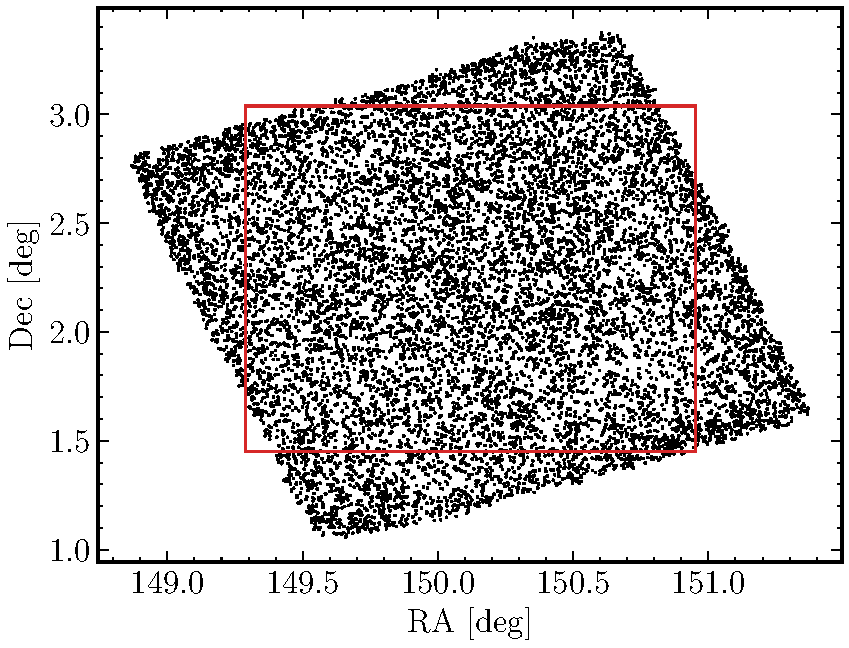
\includegraphics[width=0.75\columnwidth]{Figures/sky_map.pdf}
	\caption{{\color{red} Caption.}}
	\label{fig:sky_map}
\end{figure}